%---------------------------------- Large Language Models -------------------------------
\begin{frame}{Large Language Models}
\begin{columns}
      
    \begin{column}[t]{0.5\textwidth}
    \begin{block}{Summary}
    
        \begin{itemize}
            \item State-of-the-art of Natural Language Processing (NLP) problems
            \item Architecture : Transformers\cite{NIPS2017_3f5ee243} block, mixed with classical layers (MLP, Conv)
        \end{itemize}
            

    \end{block}
    \end{column}
        
    \begin{column}[t]{0.5\textwidth}
    \begin{block}{Self Attention cell}

        \begin{figure}
            \centering
            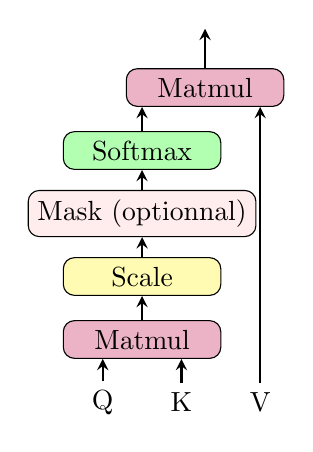
\begin{tikzpicture}[node distance=0.8cm]

\tikzstyle{matmul} = [rectangle,rounded corners, minimum width=2cm , text centered, draw=black, fill=purple!30]
\tikzstyle{softmax} = [rectangle,rounded corners, minimum width=2cm , text centered, draw=black, fill=green!30]
\tikzstyle{mask} = [rectangle,rounded corners, minimum width=2cm , text centered, draw=black, fill=pink!30]
\tikzstyle{sca} = [rectangle, rounded corners, minimum width=2cm ,text centered, draw=black, fill=yellow!30]
\tikzstyle{action} = [rectangle, rounded corners, minimum width=2cm ,text centered, draw=black, fill=red!30]
\tikzstyle{arrow} = [thick,->,>=stealth]


% Define nodes
\node (matmul1) [matmul]{Matmul};
\node (softmax)[softmax, below of = matmul1, xshift = -0.8cm]{Softmax};
\node (mask) [mask, below of=softmax]{Mask (optionnal)};
\node (scale) [sca, below of=mask]{Scale};
\node (matmul2) [matmul, below of=scale]{Matmul};
\node (q) [below of=matmul2, xshift=-0.5cm]{Q};
\node (k) [below of=matmul2, xshift=0.5cm]{K};
\node (v) [below of=matmul2, xshift=1.5cm]{V};


% Draw arrows
\draw [arrow] (matmul1.north) -- ([yshift=0.5cm]matmul1.north);
\draw [arrow] (softmax.north) -- ([xshift=-0.8cm]matmul1.south);
\draw [arrow] (mask.north) -- (softmax.south);
\draw [arrow] (scale.north) -- (mask.south);
\draw [arrow] (matmul2.north) -- (scale.south);
\draw [arrow] (q.north) -- ([xshift=-0.5cm]matmul2.south);
\draw [arrow] (k.north) -- ([xshift=0.5cm]matmul2.south);
\draw [arrow] (v.north) -- ([xshift=0.7cm]matmul1.south);



\end{tikzpicture}
            \caption{Scaled dot product attention}
        \end{figure}
    

    \end{block}
    \end{column}
         
\end{columns}
\end{frame}

%---------------------------------- Self attention mecanism -------------------------------

\begin{frame}{mha}
    \begin{figure}
        \centering
        \begin{tikzpicture}[node distance=0.8cm]

\tikzstyle{matmul} = [rectangle,rounded corners, minimum width=2cm , text centered, draw=black, fill=purple!30]
\tikzstyle{softmax} = [rectangle,rounded corners, minimum width=2cm , text centered, draw=black, fill=green!30]
\tikzstyle{mask} = [rectangle,rounded corners, minimum width=2cm , text centered, draw=black, fill=pink!30]
\tikzstyle{sca} = [rectangle, rounded corners, minimum width=2cm ,text centered, draw=black, fill=yellow!30]
\tikzstyle{action} = [rectangle, rounded corners, minimum width=2cm ,text centered, draw=black, fill=red!30]
\tikzstyle{arrow} = [thick,->,>=stealth]

\tikzstyle{linear} = [rectangle, rounded corners, minimum width=1cm ,text centered, draw=black, fill=blue!30]
\tikzstyle{dot-prod} = [rectangle, rounded corners, minimum width=2cm,minimum height = 1cm ,text centered, draw=black, fill=purple!50]
\tikzstyle{concat} = [rectangle, rounded corners, minimum width=2cm ,text centered, draw=black, fill=yellow!50]



% Define nodes
\node (matmul1) [matmul]{Matmul};
\node (softmax)[softmax, below of = matmul1, xshift = -0.8cm]{Softmax};
\node (mask) [mask, below of=softmax]{Mask (optionnal)};
\node (scale) [sca, below of=mask]{Scale};
\node (matmul2) [matmul, below of=scale]{Matmul};
\node (q) [below of=matmul2, xshift=-0.5cm]{Q};
\node (k) [below of=matmul2, xshift=0.5cm]{K};
\node (v) [below of=matmul2, xshift=1.5cm]{V};


% Draw arrows
\draw [arrow] (matmul1.north) -- ([yshift=0.5cm]matmul1.north);
\draw [arrow] (softmax.north) -- ([xshift=-0.8cm]matmul1.south);
\draw [arrow] (mask.north) -- (softmax.south);
\draw [arrow] (scale.north) -- (mask.south);
\draw [arrow] (matmul2.north) -- (scale.south);
\draw [arrow] (q.north) -- ([xshift=-0.5cm]matmul2.south);
\draw [arrow] (k.north) -- ([xshift=0.5cm]matmul2.south);
\draw [arrow] (v.north) -- ([xshift=0.7cm]matmul1.south);


% MHA 
\node (linear1) [linear, right of = matmul1, xshift = 4cm] {Linear};
\node (concat) [concat, below of = linear1] {Concat};
\node (dot-prod) [dot-prod, below of = concat,yshift= -0.4cm] {Scaled Dot-product Attention};
\node (linear2) [linear, below of = dot-prod, xshift = -1.5cm, yshift = -0.4cm] {Linear};
\node (linear3) [linear, below of = dot-prod, yshift = -0.4cm] {Linear};
\node (linear4) [linear, below of = dot-prod, xshift = 1.5cm, yshift = -0.4cm] {Linear};
\node (q2) [below of=linear2]{Q};
\node (k2) [below of=linear3]{K};
\node (v2) [below of=linear4]{V};

% MHA arrow
\draw [arrow] (q2) -- (linear2);
\draw [arrow] (k2) -- (linear3);
\draw [arrow] (v2) -- (linear4);
\draw [arrow] (linear2.north) -- ([xshift=-1.5cm]dot-prod.south);
\draw [arrow] (linear3.north) -- (dot-prod.south);
\draw [arrow] (linear4.north) -- ([xshift=1.5cm]dot-prod.south);
\draw [arrow] (dot-prod) -- (concat);
\draw [arrow] (concat) -- (linear1);
\draw [arrow] (linear1.north) -- ([yshift=0.5cm]linear1.north);

% MHA * h
\node[draw, thick, dashed, rounded corners, fit=(dot-prod), inner sep=0.1cm, label=right:{$\times$ h}] {};
\node[draw, thick, dashed, rounded corners, fit=(linear2)(linear3)(linear4), inner sep=0.1cm, label=right:{$\times$ h}] {};


% Title
\node (dot_t) [above of = matmul1,yshift=0.5cm] {\textbf{Scaled Dot-Product Attention}};
\node (mha) [above of = linear1,yshift=0.5cm] {\textbf{Multi-Head Attention}};



\end{tikzpicture}
        \caption{MHA}
    \end{figure}  
        

    
\end{frame}


%---------------------------------- Self attention mecanism -------------------------------

\begin{frame}{self attention}
    \begin{figure}
        \centering
        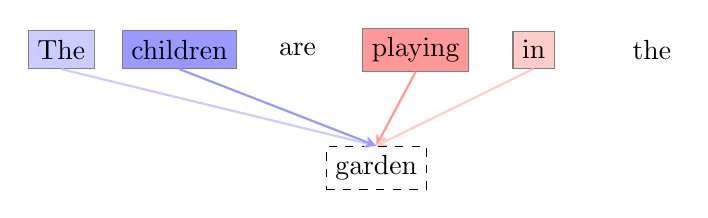
\begin{tikzpicture}[node distance=1.5cm]

% Define block styles
\tikzstyle{model} = [rectangle,rounded corners, minimum width=2cm, minimum height=1cm, text centered, draw=black, fill=blue!30]
\tikzstyle{arrow} = [thick,->,>=stealth]

% Define nodes
\node (the) [fill=blue!20,rectangle,draw=black!50] {The};
\node (children) [right of = the,fill=blue!40,rectangle,draw=black!50] {children};
\node (are) [right of = children] {are};
\node (playing) [right of = are,fill=red!40,rectangle,draw=black!50] {playing};
\node (in) [right of = playing,fill=red!20,rectangle,draw=black!50] {in};
\node (the2) [right of = in] {the};

\node (garden) [below of = are, xshift=1cm,rectangle,dashed,draw=black] {garden};

% Draw arrows
\draw [arrow,draw=blue!20] (the.south) -- (garden.north);
\draw [arrow,draw=blue!40] (children.south) -- (garden.north);
\draw [arrow,draw=red!40] (playing.south) -- (garden.north);
\draw [arrow,draw=red!20] (in.south) -- (garden.north);

% Add a rectangle around the last four nodes
\end{tikzpicture}
        \caption{self attention mecanism}
    \end{figure}  
        

    
\end{frame}


%---------------------------------- Transformers -------------------------------

\begin{frame}{Pre-training and Fine-tuning}
    \begin{figure}
        \centering
        \begin{tikzpicture}[node distance=1.5cm]

% Define block styles
\tikzstyle{model} = [rectangle,rounded corners, minimum width=2cm, minimum height=1cm, text centered, draw=black, fill=blue!30]
\tikzstyle{data} = [rectangle, rounded corners, minimum width=2cm, minimum height=1cm,text centered, draw=black, fill=yellow!30]
\tikzstyle{action} = [rectangle, rounded corners, minimum width=2cm, minimum height=1cm,text centered, draw=black, fill=red!30]
\tikzstyle{arrow} = [thick,->,>=stealth]

% Define nodes
\node (model1) [model,align=center] {Model\\Random init};
\node (data1) [data, below of=model1,align=center]{Pre-Training \\ Data Corpus} ;
\node (pre-train)[action, right of=model1, xshift=1.5cm,yshift=-1cm]{Pre-Training};
\node (model2) [model, right of=pre-train, xshift = 1.5cm, yshift=1cm ]{Pre-Trained Model};
\node (data2) [data, below of= model2]{In-domain data};
\node (fine-tuning)[action, right of = model2, xshift = 1.5cm,yshift=-1cm]{Fine Tuning};
\node (model3) [model, right of=fine-tuning, xshift = 1.5cm,align=center ]{Fine-Tuned \\ model};


% Draw arrows
\draw [arrow] (data1) -- (pre-train);
\draw [arrow] (model1) -- (pre-train);
\draw [arrow] (pre-train) -- (model2);
\draw [arrow] (model2) -- (fine-tuning);
\draw [arrow] (data2) -- (fine-tuning);
\draw [arrow] (fine-tuning) -- (model3);

% Add a rectangle around the last four nodes
\node[draw, thick, dashed, rounded corners, fit=(model2) (fine-tuning) (model3) (data2), inner sep=0.5cm, label=above:{Fine-Tuning Framework}] {};
\end{tikzpicture}
        \caption{Pre-training and Fine-tuning generic workflow}
    \end{figure}  
        

    
\end{frame}


%---------------------------------- Fine Tuning Frame -------------------------------
\begin{frame}{Fine Tuning}

   \begin{block}{Instruction Tuning}
       fine-tunes models to follow specific user instructions effectively. Consists of using specific fine-tuning datasets (Alpaca \cite{alpaca}, Databrick's Dolly\cite{DatabricksBlog2023DollyV2})   
    \end{block}



    \begin{block}{Parameters Efficient Fine-Tuning (PEFT)}
    Set of methods aims to reduce the computation cost of fine-tuning. Can change the structure like the 2 following, or just reduce the cost like Quantization (reduce the precision of calculus). These methods are often hyperparameter-dependent.     
    \end{block}
    
    \begin{columns}  
  
        \begin{column}[t]{0.45\textwidth}
        \begin{block}{Low Rank Adaptation (LoRA)\cite{hu2021loralowrankadaptationlarge}}
                   Use of low rank matrices of the weights matrices, which will be the only ones trained, to reduce the cost of gradient computations.  
        \end{block}
        \end{column}
    
        \begin{column}[t]{0.45\textwidth}
        \begin{block}{Adapter Layer}
            Add layer inside the model, and train only these. One con is to add inference for predicting.
            
        \end{block}
        \end{column}
      
    \end{columns}

\end{frame}

%---------------------------------- LoRA -------------------------------
\begin{frame}{Low Rank Adaptation (LoRA)}
    \begin{block}{Principle}
        Merging Fine-tuning layers with pre-trained ones can be written as $W = W_0 + \Delta W$, with $W_0$ the pre-trained weights and $\Delta W$ the fine-tuned ones.         
    \end{block}

    \begin{columns}
        \begin{column}[t]{0.45\textwidth}
        \begin{figure}
            \centering
            %\includegraphics[width=0.5\linewidth]{imgs/lora.png}
            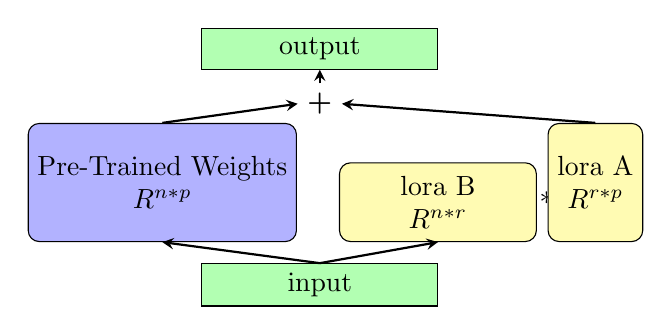
\begin{tikzpicture}[node distance=1.5cm]
    % Define block styles
    \tikzstyle{weights} = [rectangle,rounded corners, minimum width=2.5cm, minimum height=1.5cm, text centered, draw=black, fill=blue!30]
    \tikzstyle{lora_a} = [rectangle,rounded corners, minimum width=1cm, minimum height=1.5cm, text centered, draw=black, fill=yellow!30]
    \tikzstyle{lora_b} = [rectangle,rounded corners, minimum width=2.5cm, minimum height=1cm, text centered, draw=black, fill=yellow!30]
    \tikzstyle{vector} = [rectangle, minimum width=3cm, minimum height=0.5cm, text centered, draw=black, fill=green!30]
    \tikzstyle{arrow} = [thick,->,>=stealth]
    
    % Define nodes
    \node (weights) [weights, align=center]{Pre-Trained Weights \\ $\mathbb{R}^{n*p}$};
    \node (lora_B) [lora_b, right of=weights,xshift=2cm,yshift=-0.25cm, align=center]{lora B\\ $\mathbb{R}^{n*r}$};
    \node (mul) [right of = lora_B,xshift=-0.12cm]{*};
    \node (lora_A) [lora_a, right of=lora_B,xshift=0.5cm,yshift=0.25cm, align=center]{lora A\\$\mathbb{R}^{r*p}$};
    \node (input) [vector,below of = weights, xshift = 2cm,yshift=+0.2cm]{input};
    \node (plus) [above of = weights, xshift = 2cm,yshift=-0.5cm]{\textbf{+}};
    \node (output) [vector,above of = plus,yshift=-0.8cm]{output};
    
    
    
    
    % Draw arrows
    \draw [arrow] (input.north) -- (weights.south);
    \draw [arrow] (input.north) -- (lora_B.south);
    \draw [arrow] (weights.north) -- (plus.west);
    \draw [arrow] (lora_A.north) -- (plus.east);
    \draw [arrow] (plus) -- (output);
    
    
    \end{tikzpicture}
            \caption{LoRA Decomposition}
        \end{figure}
            
        \end{column}
        
        \begin{column}[t]{0.3\textwidth}
            \begin{block}{LoRA hyperparameters}
            \begin{itemize}
                \item rank : the common dimension between $A$ and $B$.
                \item alpha : apply a weighting between fine-tuning and pre-trained weights
            \end{itemize}
                
            \end{block}
            
        \end{column}
    \end{columns}
    
\end{frame}

%---------------------------------- Hyper-Parameter Optimization -------------------------------
\begin{frame}[allowframebreaks]{Hyper-Parameter Optimization (HPO)}
    
    \begin{columns}
    
        \begin{column}[t]{0.45\textwidth}
        \begin{block}{Hyper-Parameters}
            In a Deep Learning Context, set of value that the algorithms need to run. Affect the model, the training or the prediction. The hyper-parameters, often called variables, are mixed (i.e. continuous and integers, no categoricals).
        \end{block}
        \end{column}
        
        \begin{column}[t]{0.45\textwidth}
        \begin{block}{Optimization}
            Set of methods to find the best input value to maximize or minimize an objective function. The problem here can be defined as a black-box optimization (i.e. no analytic form), and an expensive one. An evaluation can take hours.
        \end{block}
        \end{column}
         
  \end{columns}

    \vspace{1cm}
  
      \noindent The Hyper-Parameter Optimization field can be defined as the use of Optimization method to hyper-parameter dependent problem, like Deep Learning ones.\\
      Aims are diverses, from obtaining better results, putting humans out of the loop or ensuring reliability.

\framebreak

\begin{block}{Generic workflow}
    \begin{figure}
        \centering
        \includegraphics[width=0.4\linewidth]{imgs/hpo_workflow.png}
        \caption{HPO Workflow}
    \end{figure}

    
\end{block}
\end{frame}